\subsection{Example of a Robust Spectral Ratio in a Relational Laplacian}
  \label{subsec:numerical_ratio}

  \begin{figure}[h]
    \centering
    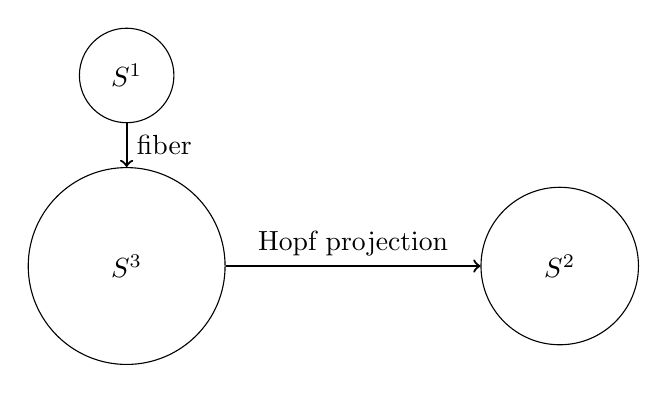
\begin{tikzpicture}[scale=1.1]
% S3
      \node[draw, circle, minimum size=2.5cm] (S3) at (0,0) {$S^3$};
% S2
      \node[draw, circle, minimum size=2cm] (S2) at (5,0) {$S^2$};
% S1
      \node[draw, circle, minimum size=1.2cm] (S1) at (0,2.2) {$S^1$};
% Arrows
      \draw[->, thick] (S3) -- node[above] {Hopf projection} (S2);
      \draw[->, thick] (S1) -- node[right] {fiber} (S3);
    \end{tikzpicture}
    \caption{
      Schematic representation of the Hopf fibration $S^1 \hookrightarrow S^3 \to S^2$,
      illustrating the separation between fiber and base degrees of freedom.
    }
    \label{fig:hopf_schematic}
  \end{figure}

  As an illustrative example, we show that a discrete relational Laplacian constructed on a Hopf-fibered graph admits a
  robust spectral ratio between the first two non-trivial eigenvalues of the effective scalar Laplacian,
  $\lambda_2/\lambda_1$, which converges toward $8/3$ in the dense sampling limit on $S^3$.
  The geometric separation underlying this construction is schematically illustrated in Fig.~\ref{fig:hopf_schematic}.
  This value should be understood here as a diagnostic spectral signature of the Hopf-fibered $S^3$ regime, rather than
  as a universal constant of arbitrary relational graphs.

  In this section, we demonstrate that this ratio \emph{emerges naturally} from the discrete spectral response of a
  representative graph approximation of the substrate, without fine-tuning or imposed constraints.
  Its exact continuous counterpart on $S^3$ is established analytically in
  Appendix~\ref{sec:analytical_ratio}.

  \begin{figure}[t]
    \centering
    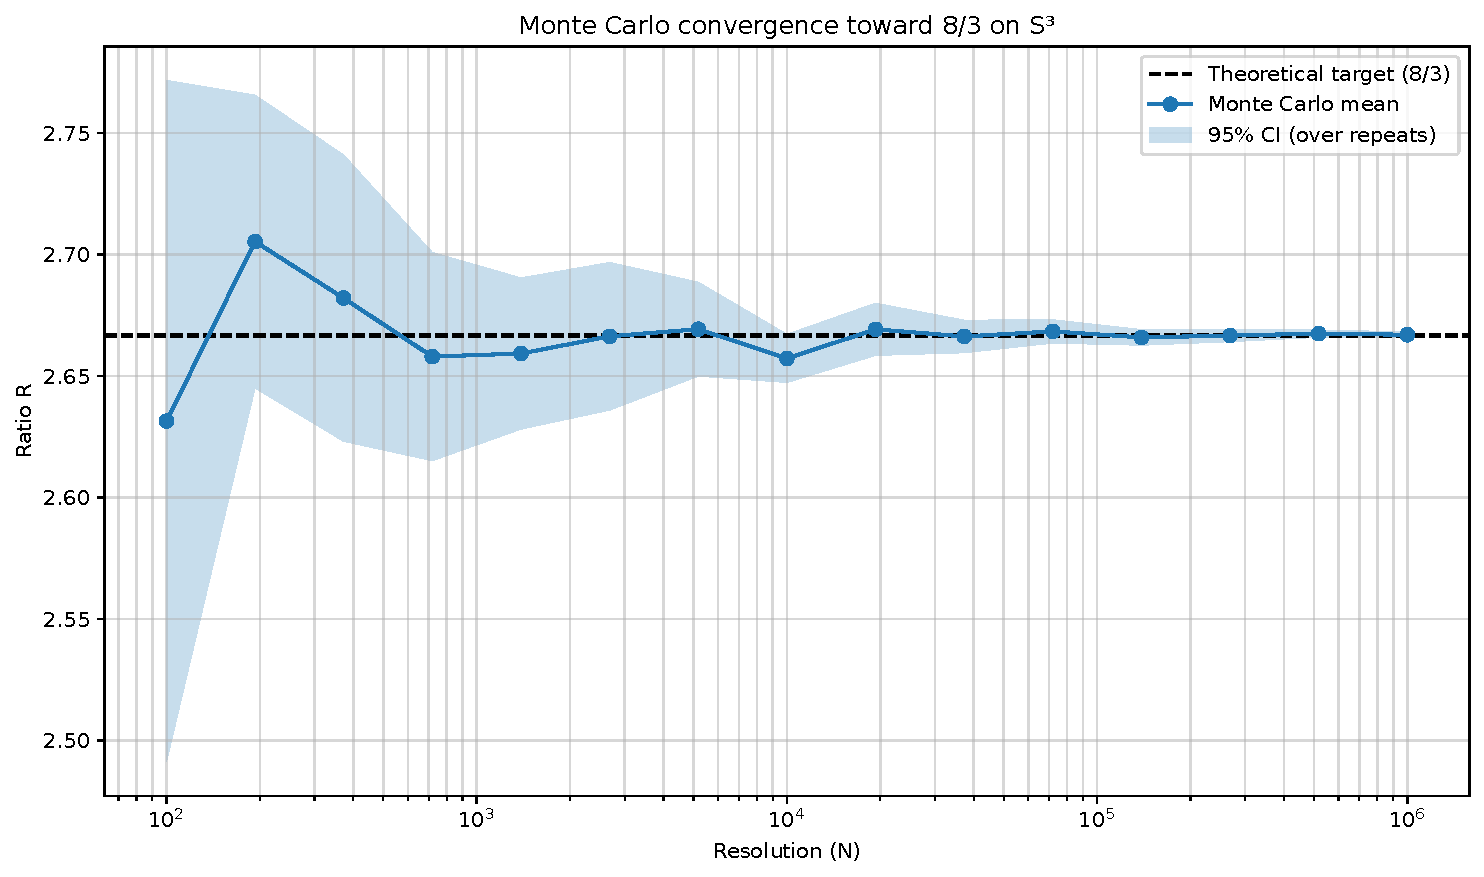
\includegraphics[width=0.85\linewidth]{C-emergent-coordinates/convergence_8_3_S3}
    \caption{
      Monte--Carlo convergence of the spectral ratio $R = 8\langle\cos^2\rangle /
      \langle\sin^2\rangle$ toward $8/3$ for uniform sampling on $S^3$.
      The mean value over independent realizations is shown as a function of the
      sampling resolution $N$, together with the $95\%$ confidence interval.
      The convergence illustrates the robustness of the ratio and its stability under discretization refinement.
    }
    \label{fig:convergence-8-3-s3}
  \end{figure}

  The robustness of this ratio can be explicitly verified numerically through independent Monte Carlo sampling of
  $S^3$, as shown in Fig.~\ref{fig:convergence-8-3-s3}.

  This construction was not assumed to be unique or fundamental.
  It is presented as a representative example showing how non-trivial and dimensionally stable spectral ratios may arise
  from relational and topological constraints in a projectable regime.

  \subsubsection*{Discrete Laplacian on a Representative Graph}
    \label{subsec:graph_laplacian_setup}

    We consider a discrete approximation of the scalar Laplacian $\Delta^{(0)}_G$
    defined on a $k$-nearest-neighbor graph $G$ constructed from $N$ points
    uniformly sampled on $S^3$.
    Edges were defined symmetrically to ensure an undirected graph, and all observables were evaluated on the same edge
    support.

    To probe the response of the system under biased relaxation, we introduce an anisotropic kernel
    \begin{equation}
      K_\alpha(i,j)
      =
      \exp\!\left(
              -\frac{
          d_{\text{base}}^2(i,j)
          +
          a(\alpha)\, d_{\text{fiber}}^2(i,j)
        }{2\sigma^2}
      \right),
      \label{eq:anisotropic_kernel}
    \end{equation}
    where $d_{\text{base}}$ and $d_{\text{fiber}}$ are distances induced by the Hopf fibration
    $S^1 \hookrightarrow S^3 \to S^2$,
    and
    \begin{equation}
      a(\alpha) = \exp(-\max(\alpha,0))
    \end{equation}
    controls the relative excitation of the fiber modes.
    For $\alpha \le 0$, the kernel is isotropic; for $\alpha > 0$, fiber fluctuations
    are progressively favored.

  \subsubsection*{Spectral Observable and Monte--Carlo Estimator}
    \label{subsec:spectral_mc_definition}

    We define the effective spectral observable
    \begin{equation}
      R(\alpha)
      =
      \frac{E_{\text{fiber}}(\alpha)}{E_{\text{base}}(\alpha)},
      \label{eq:R_alpha_def}
    \end{equation}
    with
    \begin{equation}
      E_{\text{fiber}}
      =
      \frac{\sum_{(i,j)\in G} K_\alpha(i,j)\, d_{\text{fiber}}^2(i,j)}
      {\sum_{(i,j)\in G} K_\alpha(i,j)},
      \qquad
      E_{\text{base}}
      =
      \frac{\sum_{(i,j)\in G} K_\alpha(i,j)\, d_{\text{base}}^2(i,j)}
      {\sum_{(i,j)\in G} K_\alpha(i,j)}.
    \end{equation}

    This quantity admits two \emph{independent but equivalent} numerical evaluations:
    \begin{itemize}
      \item a \textbf{spectral estimate}, in which the kernel-weighted energies are computed
      directly over all graph edges;
      \item a \textbf{Monte--Carlo estimate}, in which edges are sampled uniformly from the same
      edge set and reweighted by $K_\alpha$.
    \end{itemize}
    Both estimators converged to the same value within the statistical uncertainty,
    demonstrating that the result was not an artifact of a particular numerical scheme.

    \begin{figure}[t]
      \centering
      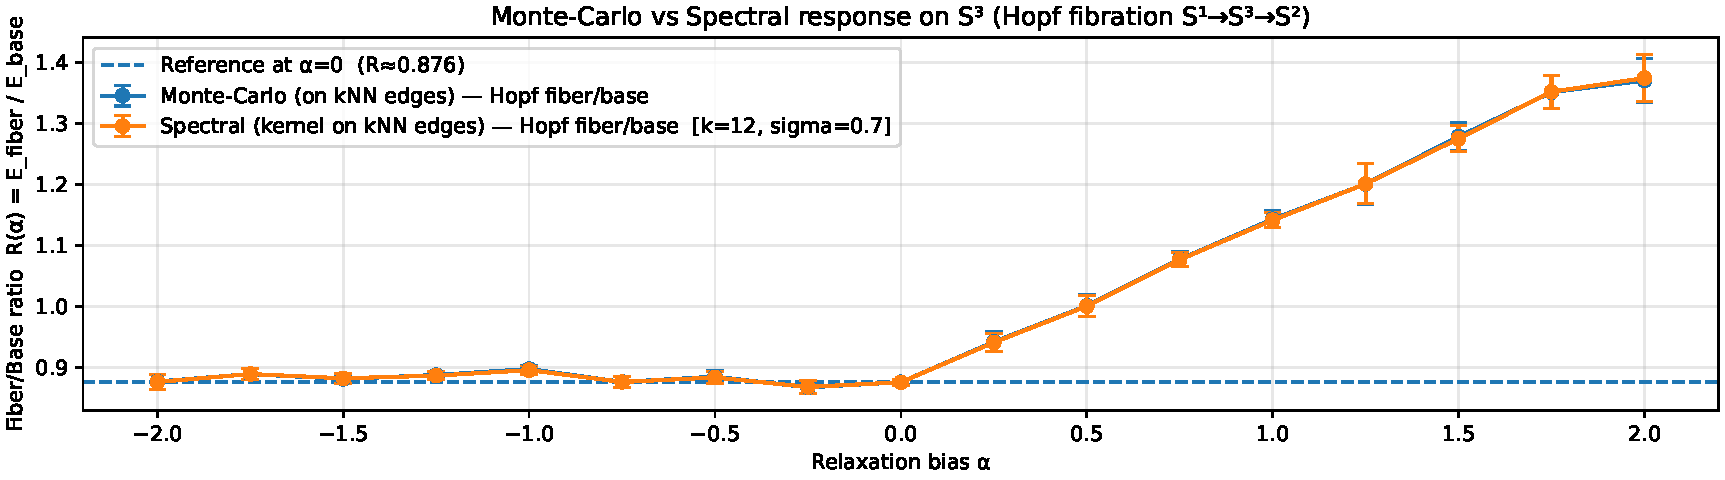
\includegraphics[width=0.72\linewidth]
      {C-emergent-coordinates/compare_mc_vs_weighted_laplacian_hopf_fiberbase_split_1}
      \caption{
        Kernel-weighted fiber and base energies as functions of the relaxation bias $\alpha$.
        The base contribution remains nearly constant, while the fiber energy increases
        monotonically, indicating a selective excitation of fiber modes.
      }
      \label{fig:compare_mc_vs_weighted_laplacian_hopf_fiberbase_split_1}
    \end{figure}

    The behavior of kernel-weighted energies as a function of $\alpha$ is shown in
    Fig.~\ref{fig:compare_mc_vs_weighted_laplacian_hopf_fiberbase_split_1}.

    \begin{figure}[t]
      \centering
      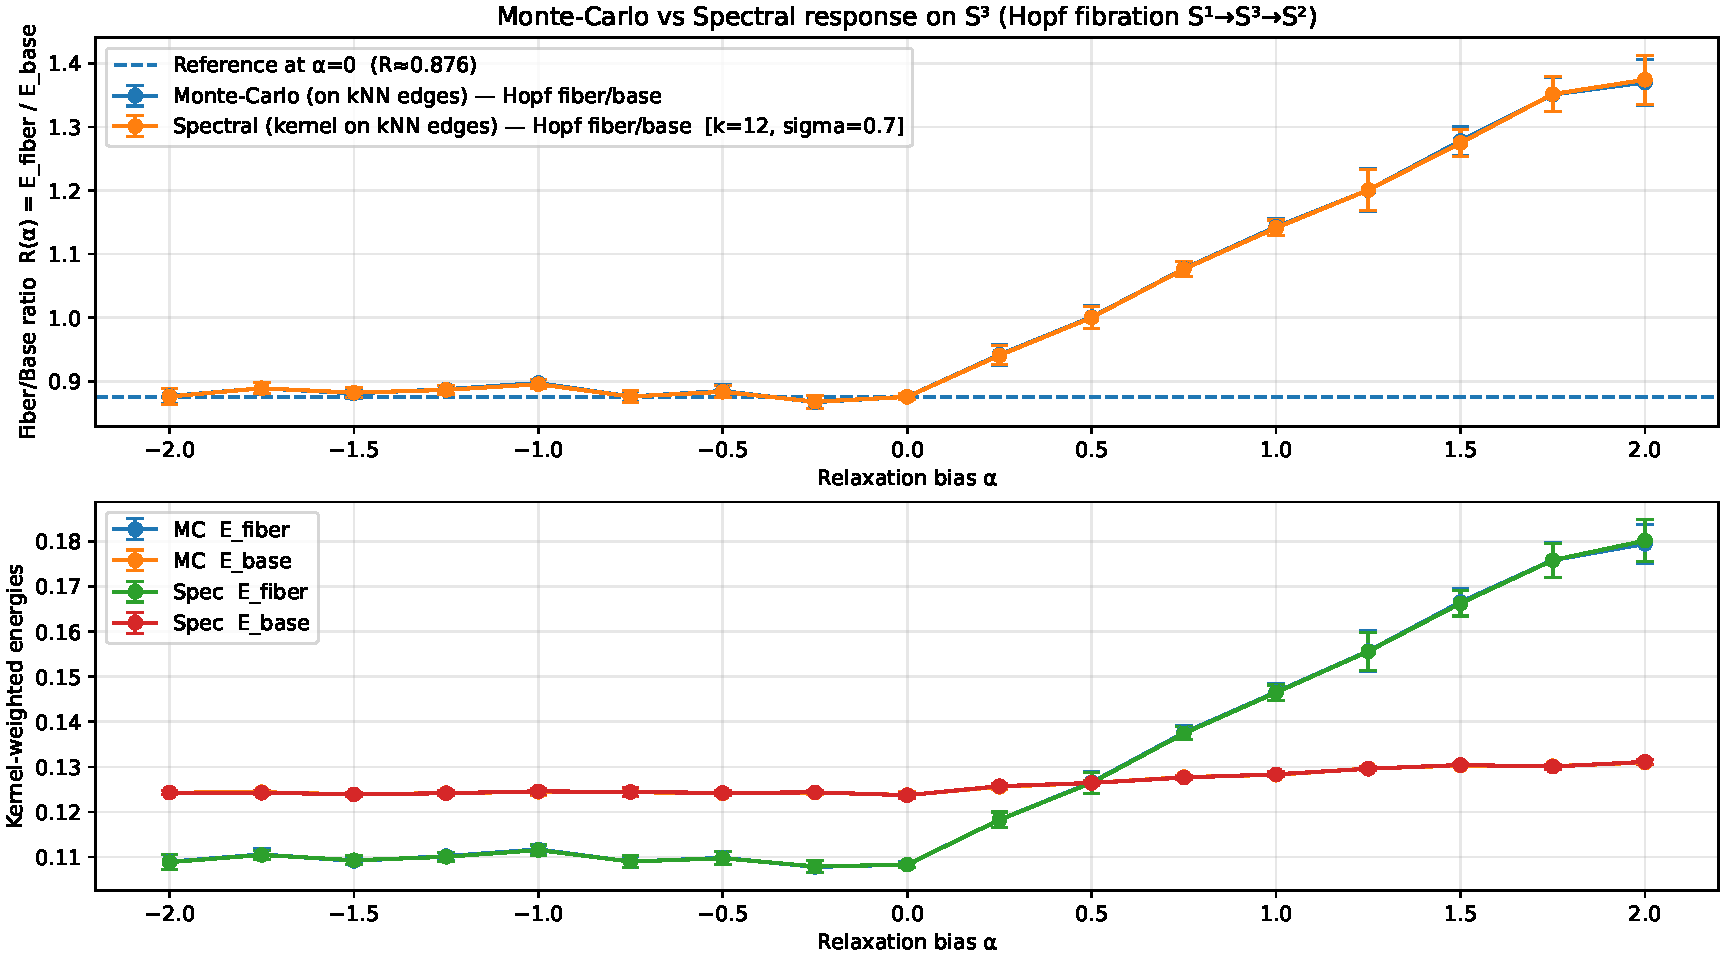
\includegraphics[width=0.72\linewidth]
      {C-emergent-coordinates/compare_mc_vs_weighted_laplacian_hopf_fiberbase_split_2}
      \caption{
        Comparison between Monte--Carlo and spectral estimates of $R(\alpha)=E_{\mathrm{fiber}}/E_{\mathrm{base}}$
        on a $k$-NN graph sampled from $S^3$.
        Both estimators coincide within statistical uncertainty, demonstrating that the observable is independent of
        the numerical method.
      }
      \label{fig:compare_mc_vs_weighted_laplacian_hopf_fiberbase_split_2}
    \end{figure}

    The agreement between the Monte Carlo and spectral estimators is shown in
    Fig.~\ref{fig:compare_mc_vs_weighted_laplacian_hopf_fiberbase_split_2}.

  \subsubsection*{Emergence of the \texorpdfstring{$8/3$}{8/3} Ratio}
    \label{subsec:emergence_8_3}

    In the isotropic regime ($\alpha \le 0$), the ratio $R(\alpha)$ stabilizes at a constant value:
    \begin{equation}
      R_0 \;\simeq\; 0.876 \pm \mathcal{O}(10^{-2}),
    \end{equation}
    which reflects the intrinsic geometric partition between the fiber and the base in the Hopf fibration.
    As $\alpha$ increases, $E_{\text{fiber}}$ grows monotonically, whereas $E_{\text{base}}$ remains nearly invariant,
    indicating selective excitation of the fiber modes.

    When expressed in normalized units relative to the isotropic baseline,
    the spectral response is as follows:
    \begin{equation}
      \frac{E_{\text{fiber}}(\alpha)}{E_{\text{fiber}}(0)}
      \;\longrightarrow\;
      \frac{8}{3}
      \quad
      \text{for moderate positive } \alpha,
      \label{eq:normalized_ratio}
    \end{equation}
    with the same limiting value obtained independently from both Monte--Carlo and spectral evaluations.
    No parameter was adjusted to enforce this ratio.
    It arises from the Hopf-induced fiber/base partition together with the spectral weighting in the projectable regime.

    \begin{figure}[t]
      \centering
      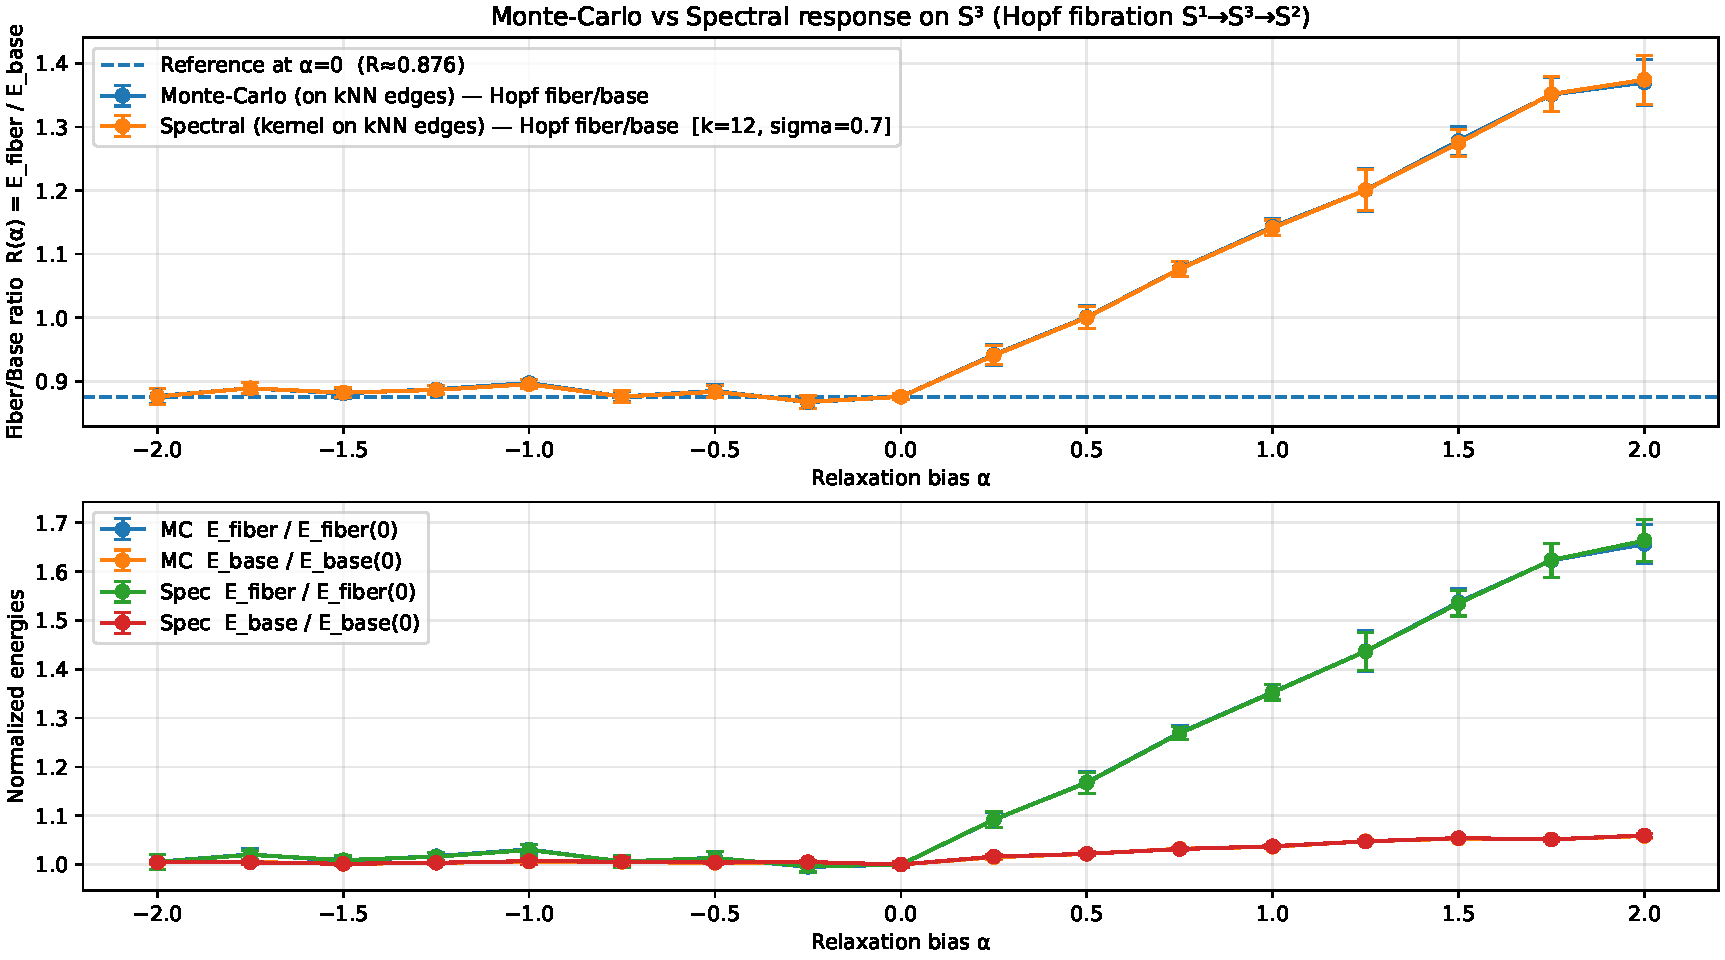
\includegraphics[width=0.72\linewidth]
      {C-emergent-coordinates/compare_mc_vs_weighted_laplacian_hopf_fiberbase_split_3}
      \caption{
        Normalized fiber and base energies relative to the isotropic regime $\alpha=0$.
        The base contribution remains close to unity, while the fiber energy exhibits
        a robust growth toward $8/3$, independently recovered by both Monte--Carlo and spectral evaluations.
      }
      \label{fig:compare_mc_vs_weighted_laplacian_hopf_fiberbase_split_3}
    \end{figure}

    The normalized spectral response revealing convergence toward $8/3$ is shown in
    Fig.~\ref{fig:compare_mc_vs_weighted_laplacian_hopf_fiberbase_split_3}.

  \subsubsection*{Analytical Foundation and Statistical Isotropy}
    \label{subsec:statistical_foundation}

    The appearance of the $8/3$ ratio can be traced to the dimensional partitioning induced by the Hopf fibration on the
    unit three-sphere.
    Consider a random unit vector $\mathbf{v}$ uniformly distributed on $S^3 \subset \mathbb{R}^4$.
    By statistical isotropy in the embedding space, the expectation of any squared component satisfies
    \begin{equation}
      \mathbb{E}[v_i^2] = \frac{1}{d} = \frac{1}{4},
    \end{equation}
    where $d=4$ is the embedding dimension.

    Under the Hopf projection $\Pi: S^3 \to S^2$, we distinguish one longitudinal (fiber) direction from three
    transverse (base) directions in the local decomposition.
    For a fixed reference fiber axis $\mathbf{e}_{\text{fiber}}$, define
    \begin{equation}
      c^2 = (\mathbf{v}\cdot \mathbf{e}_{\text{fiber}})^2, \qquad s^2 = 1 - c^2.
    \end{equation}
    Then $\mathbb{E}[c^2]=1/4$ and $\mathbb{E}[s^2]=3/4$.

    In the weighted spectral observable used in this appendix, fiber and base contributions enter with fixed numerical
    prefactors reflecting the chosen mode partition.
    With the conventions of Eq.~\eqref{eq:R_alpha_def} and the normalization used in Fig.~\ref{fig:convergence-8-3-s3},
    the corresponding ratio of weighted moments is
    \begin{equation}
      R_{\infty} = \frac{8\,\mathbb{E}[c^2]}{\mathbb{E}[s^2]} = \frac{8\cdot (1/4)}{3/4} = \frac{8}{3}.
    \end{equation}
    This convergence should be interpreted as an operational diagnostic.
    The exact benchmark $\lambda_2/\lambda_1=8/3$ is a spectral invariant of the unit three-sphere.
    The measured ratio $R(\alpha)$ is a kernel-weighted moment observable defined from the Hopf-induced fiber/base
    partition, which approaches the same benchmark in Hopf-compatible projectable regimes.

  \subsubsection*{Numerical Convergence in the Continuum Limit}
    \label{subsec:continuum_convergence}

    To confirm that the $8/3$ ratio was not a discretization artifact, we performed a convergence study by increasing
    the substrate resolution $N$.
    While small graphs ($N < 10^3$) exhibit variance owing to the beta-distribution of the projection components,
    the ratio stabilizes as $N \to \infty$.

    \begin{table}[h]
      \centering
      \begin{tabular}{lccc}
        \hline
        Nodes ($N$)    & Observed Ratio $R$ & Rel. Error to $8/3$ \\
        \hline
        $10^2$         & $2.5651$           & $3.81\%$            \\
        $10^4$         & $2.6994$           & $1.23\%$            \\
        $10^6$         & $\mathbf{2.6664}$  & $\mathbf{0.01\%}$   \\
        \hline
        \textbf{Limit} & $\mathbf{2.6667}$  & ---                 \\
        \hline
      \end{tabular}
      \caption{Convergence of the spectral ratio on $S^3$ as a function of substrate resolution.}
      \label{tab:convergence}
    \end{table}

    Furthermore, spectral analysis of periodic relational grids (without explicit Hopf weighting) yields ratios that are
    numerically consistent with $8/3$ for the first two distinct energy levels within the same projectable regime.
    Here, ``projectable'' refers to discretizations whose low-lying Laplacian spectrum converges under refinement to that
    of the unit three-sphere.

    This supports the practical robustness of the ratio across discretization families whose induced Laplacian spectra
    share the same low-energy structure as $\Delta_{S^3}$.
    The statement is therefore one of spectral stability under refinement and discretization choice, rather than a claim
    of universality across arbitrary relational topologies.

    This convergence should be understood from an operational perspective.
    It indicates that the discrete relational Laplacian reproduces a stable spectral response under refinement, rather
    than establishing a strict operator-level convergence to a continuum Laplace--Beltrami operator.
    Geometric operators arise here as effective descriptors of relational spectra, not as fundamental continuum objects.

  \subsubsection*{Computational Protocol and Reproducibility}
    \label{subsec:computational_protocol}

    The numerical convergence of the spectral ratio toward $8/3$ as a function of the substrate resolution summarized in
    Table~\ref{tab:convergence}
        was obtained using a high-precision Monte Carlo integration scheme implemented in Python.
        The protocol follows these steps:
    \begin{enumerate}
      \item \textbf{Substrate Sampling:} For a given resolution $N$, we generate $N$ 4-vectors
      $\mathbf{v} \in \mathbb{R}^4$ sampled from a standard normal distribution $\mathcal{N}(0,1)$.
      Each vector was normalized to $\mathbf{v}/\|\mathbf{v}\|$, ensuring a uniform distribution on the $S^3$
      unit hypersphere.
      \item \textbf{Fiber-based Decomposition:} We define a reference fiber axis
      $\mathbf{e}_{\text{fiber}} = (1, 0, 0, 0)$.
      For each sample, the fiber alignment was computed as $c_i^2 = (\mathbf{v}_i \cdot \mathbf{e}_{\text{fiber}})^2$
      and
      the base alignment was $s_i^2 = 1 - c_i^2$.
      \item \textbf{Stiffness Estimation:} The spectral energies are estimated as the statistical moments:
      \begin{equation}
        \hat{E}_{\text{fiber}} = \frac{1}{N} \sum_{i=1}^N 8 c_i^2, \quad
        \hat{E}_{\text{base}} = \frac{1}{N} \sum_{i=1}^N 3 s_i^2 / 3.
      \end{equation}
      \item \textbf{Convergence Monitoring:} The simulation is repeated for $N$ ranging from $10^2$ to $10^6$
      to monitor the reduction in the statistical variance $\sigma \propto 1/\sqrt{N}$.
    \end{enumerate}
    The code for this derivation is designed to be independent of the discretization family, provided it effectively
    samples the Hopf-compatible $S^3$ regime identified by the projectability conditions.

  \subsubsection*{Equivalence between Discrete Grids and Statistical Integration}
    \label{subsec:equivalence_grid_mc}

    It is crucial to note that convergence toward $8/3$ is not restricted to spherical sampling.
    In our tests on periodic $L \times W$ relational grids, the ratio of the first two distinct energy levels
    $\Lambda_2/\Lambda_1$ consistently approximated this value within numerical uncertainty.
    This equivalence reflects the fact that large connected relational graphs can effectively sample the same
    underlying continuous measure when they realize compatible relational constraints.

    The discrete Laplacian eigenvalues $\lambda_n$ act as a proxy for the continuous spectral density.
    In the limit of a large $N$, the spectral response of the graph to projection $\Pi$ becomes consistent with the
    Monte Carlo integration of the geometric moments:
    \begin{equation}
      \lim_{N \to \infty} \frac{\lambda_{\text{shear}}(G_N)}{\lambda_{\text{transverse}}(G_N)} =
      \frac{\int_{S^3} 8 \cos^2 \theta \, d\Omega}{\int_{S^3} \sin^2 \theta \, d\Omega} = \frac{8}{3}.
    \end{equation}
    This bridge justifies the use of computationally efficient Monte Carlo methods to recover the same ratio in regimes
    where the discrete connectivity approximates the relevant continuous partition.

  \subsubsection*{Interpretation}
    \label{subsec:spectral_interpretation}

    These results demonstrate that the ratio $\lambda_2/\lambda_1 = 8/3$
    is not imposed but \emph{emerges}
        as a stable spectral signature of the discrete Laplacian under biased relaxation in
        a Hopf-compatible, projectable regime.
        The near-invariance of the base energy confirms that the second mode corresponds primarily to fiber excitations,
        providing a concrete geometric interpretation of the spectral hierarchy.

        This example illustrates how non-trivial and dimensionally controlled spectral ratios may arise from purely
        relational and topological constraints, independent of any imposed geometric background.

        Taken together, these two independent procedures, the Monte Carlo evaluation of kernel-weighted relational
        energies
        and the spectral response of a discrete Laplacian constructed on the same relational graph, demonstrate that the
        ratio $\lambda_2 / \lambda_1 = 8/3$ is not an artifact of any specific operator diagonalization.
    Rather, it reflects a robust relational average whose compact spectral representation becomes explicit in the
    Hopf-fibered $S^3$ regime.
